\documentclass[tikz]{standalone}
\usepackage{fontspec}
\renewcommand*{\familydefault}{\sfdefault}
\usepackage{standalone}
\usetikzlibrary{arrows.meta, decorations.pathreplacing, shapes.geometric}

\begin{document}

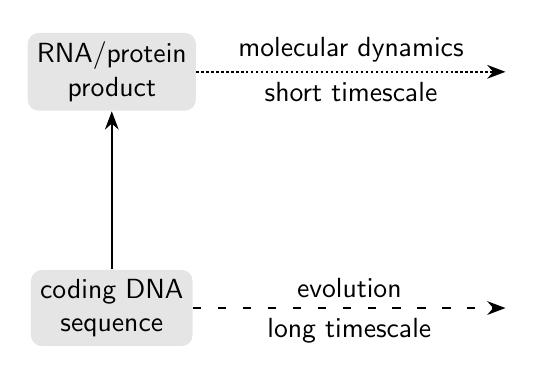
\begin{tikzpicture}

\path[rounded corners, every node/.style={fill=gray!20!white, align=center}]
(0,0) node (DNA) {coding DNA\\sequence} +(90:3 cm) node (prod) {RNA/protein\\product}
(DNA) +(0:5 cm) coordinate (D1)
(prod) +(0:5 cm) coordinate (P1)
;

\begin{scope}[-Stealth, thick]
\draw (DNA) -- (prod);
\draw[loosely dashed] (DNA) -- node[above] {evolution} node[below] {long timescale} (D1);
\draw[densely dotted] (prod) -- node[above] {molecular dynamics} node[below] {short
timescale} (P1);
%\draw[dashed] (prod) -- node[below] {long timescale} (D1);
\end{scope}

\end{tikzpicture}

\end{document}

